% ═══════════════════════════════════════════════════════════════════════════════
% Dictionary Diagram Variants — Test Document (v2, fixed layout)
% Three approaches for presenting PDF signature dictionaries with annotations
% ═══════════════════════════════════════════════════════════════════════════════
\documentclass[11pt,a4paper]{article}

\usepackage{fontspec}
\setmainfont{Noto Serif}[
    BoldFont={Noto Serif Bold},
    ItalicFont={Noto Serif Italic},
    BoldItalicFont={Noto Serif Bold Italic}
]
\setsansfont{Noto Sans}[
    BoldFont={Noto Sans Bold},
    ItalicFont={Noto Sans Italic}
]
\setmonofont{DejaVu Sans Mono}[Scale=0.82]

\usepackage[inner=0.8in,outer=0.6in,top=0.7in,bottom=0.7in]{geometry}
\usepackage{xcolor}
\usepackage{tikz}
\usetikzlibrary{
    arrows.meta, positioning, calc, decorations.pathreplacing,
    shapes.geometric, fit, backgrounds
}
\usepackage{tcolorbox}
\tcbuselibrary{breakable,skins}
\usepackage{hyperref}
\usepackage{microtype}
\usepackage{setspace}
\setstretch{1.06}
\usepackage{enumitem}
\setlist{noitemsep,topsep=2pt}

% Colors
\definecolor{accent}{HTML}{0f3460}
\definecolor{dictbg}{HTML}{1e1e2e}
\definecolor{dicttext}{HTML}{cdd6f4}
\definecolor{keycolor}{HTML}{89b4fa}
\definecolor{valcolor}{HTML}{a6e3a1}
\definecolor{commentcolor}{HTML}{6c7086}
\definecolor{annobg}{HTML}{f8f9fa}
\definecolor{annoframe}{HTML}{c9cdd4}
\definecolor{reqcolor}{HTML}{c62828}
\definecolor{optcolor}{HTML}{2e7d32}
\definecolor{condcolor}{HTML}{6a1b9a}
\definecolor{groupA}{HTML}{dbeafe}
\definecolor{groupB}{HTML}{dcfce7}
\definecolor{groupC}{HTML}{fef3c7}
\definecolor{groupD}{HTML}{fce7f3}
\definecolor{groupE}{HTML}{ede9fe}

\pagestyle{empty}

% Usable text width reference: \textwidth ≈ 17.1cm with these margins

\begin{document}

\begin{center}
{\LARGE\bfseries\sffamily\color{accent} Dictionary Diagram Variants}\\[4pt]
{\normalsize\sffamily Three layout approaches for the Signature Dictionary (\texttt{/Type /Sig})}
\end{center}

\vspace{1em}

% ═══════════════════════════════════════════════════════════════════════════════
% VARIANT A: Stacked Entry Boxes with Right-Side Annotation Arrows
% ═══════════════════════════════════════════════════════════════════════════════
\subsection*{\sffamily\color{accent} Variant A — Stacked Boxes with Arrow Annotations}

{\small Each dictionary entry is a dark horizontal bar. Annotation boxes on the right
are connected by arrows to the entries they explain.}

\vspace{0.6em}

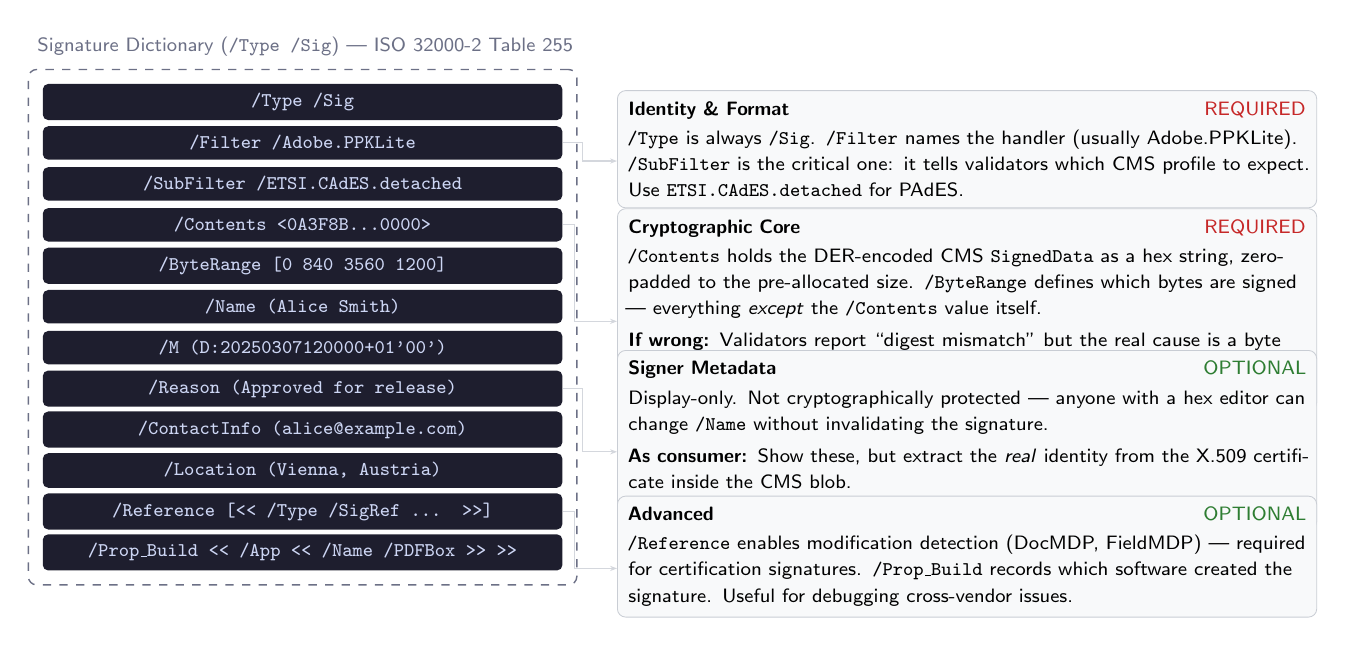
\begin{tikzpicture}[
    entry/.style={
        rectangle, rounded corners=2pt,
        fill=dictbg, text=dicttext,
        font=\fontsize{7.5}{9}\selectfont\ttfamily,
        minimum width=6.6cm, minimum height=0.42cm,
        anchor=west, inner xsep=4pt,
    },
    anno/.style={
        rectangle, rounded corners=3pt,
        fill=annobg, draw=annoframe, line width=0.3pt,
        text width=8.6cm, font=\fontsize{7.5}{9.5}\selectfont\sffamily,
        inner sep=4pt, anchor=north west,
    },
    req/.style={font=\fontsize{6}{7}\selectfont\bfseries\sffamily, text=reqcolor},
    opt/.style={font=\fontsize{6}{7}\selectfont\bfseries\sffamily, text=optcolor},
    conn/.style={draw=annoframe!80, line width=0.4pt, -{Stealth[length=2.5pt]}},
]

% Dict entries
\node[entry] (e1)  at (0, 0)     {/Type /Sig};
\node[entry] (e2)  at (0,-0.52)  {/Filter /Adobe.PPKLite};
\node[entry] (e3)  at (0,-1.04)  {/SubFilter /ETSI.CAdES.detached};
\node[entry] (e4)  at (0,-1.56)  {/Contents <0A3F8B...0000>};
\node[entry] (e5)  at (0,-2.08)  {/ByteRange [0 840 3560 1200]};
\node[entry] (e6)  at (0,-2.60)  {/Name (Alice Smith)};
\node[entry] (e7)  at (0,-3.12)  {/M (D:20250307120000+01'00')};
\node[entry] (e8)  at (0,-3.64)  {/Reason (Approved for release)};
\node[entry] (e9)  at (0,-4.16)  {/ContactInfo (alice@example.com)};
\node[entry] (e10) at (0,-4.68)  {/Location (Vienna, Austria)};
\node[entry] (e11) at (0,-5.20)  {/Reference [<< /Type /SigRef ... >>]};
\node[entry] (e12) at (0,-5.72)  {/Prop\_Build << /App << /Name /PDFBox >> >>};

% Annotations — positioned to the right, vertically aligned with their targets
\node[anno] (a1) at (7.3, 0.15) {
    \textbf{Identity \& Format} \hfill \textcolor{reqcolor}{REQUIRED}\\[1pt]
    \texttt{/Type} is always \texttt{/Sig}. \texttt{/Filter} names the handler
    (usually Adobe.PPKLite). \texttt{/SubFilter} is the critical one: it tells
    validators which CMS profile to expect. Use \texttt{ETSI.CAdES.detached} for PAdES.
};

\node[anno] (a2) at (7.3, -1.35) {
    \textbf{Cryptographic Core} \hfill \textcolor{reqcolor}{REQUIRED}\\[1pt]
    \texttt{/Contents} holds the DER-encoded CMS \texttt{SignedData} as a hex string,
    zero-padded to the pre-allocated size.
    \texttt{/ByteRange} defines which bytes are signed — everything \emph{except}
    the \texttt{/Contents} value itself.\\[2pt]
    \textbf{If wrong:} Validators report ``digest mismatch'' but the real cause is a byte
    range gap. \textbf{Fix:} Verify that \texttt{sum(all ranges) + contents\_hex\_length == file size}.
};

\node[anno] (a3) at (7.3, -3.15) {
    \textbf{Signer Metadata} \hfill \textcolor{optcolor}{OPTIONAL}\\[1pt]
    Display-only. Not cryptographically protected — anyone with a hex editor can change
    \texttt{/Name} without invalidating the signature.\\[2pt]
    \textbf{As consumer:} Show these, but extract the \emph{real} identity from the X.509
    certificate inside the CMS blob.\\
    \textbf{As producer:} Populate for convenience, but don't rely on them for security.
};

\node[anno] (a4) at (7.3, -5.0) {
    \textbf{Advanced} \hfill \textcolor{optcolor}{OPTIONAL}\\[1pt]
    \texttt{/Reference} enables modification detection (DocMDP, FieldMDP) — required for
    certification signatures. \texttt{/Prop\_Build} records which software created the
    signature. Useful for debugging cross-vendor issues.
};

% Connector arrows
\draw[conn] (e2.east) -- ++(0.25,0) |- ($(a1.west)+(0,-0.15)$);
\draw[conn] (e4.east) -- ++(0.15,0) |- ($(a2.west)+(0,-0.15)$);
\draw[conn] (e8.east) -- ++(0.25,0) |- ($(a3.west)+(0,-0.15)$);
\draw[conn] (e11.east) -- ++(0.15,0) |- ($(a4.west)+(0,-0.15)$);

% Dict frame
\begin{scope}[on background layer]
    \node[fit=(e1)(e12), inner sep=5pt, draw=commentcolor, dashed,
          rounded corners=3pt, line width=0.5pt] (frame) {};
    \node[above=1pt of frame.north west, anchor=south west,
          font=\fontsize{7}{8}\selectfont\sffamily\color{commentcolor}]
          {Signature Dictionary (\texttt{/Type /Sig}) — ISO 32000-2 Table 255};
\end{scope}

\end{tikzpicture}

\vfill
\clearpage

% ═══════════════════════════════════════════════════════════════════════════════
% VARIANT B: Color-Grouped Blocks with Side Panel
% ═══════════════════════════════════════════════════════════════════════════════
\subsection*{\sffamily\color{accent} Variant B — Color-Grouped Blocks with Side Panel}

{\small Related entries share a background color. A matching-colored explanation panel
sits on the right. The reader follows the color to find the explanation.}

\vspace{0.6em}

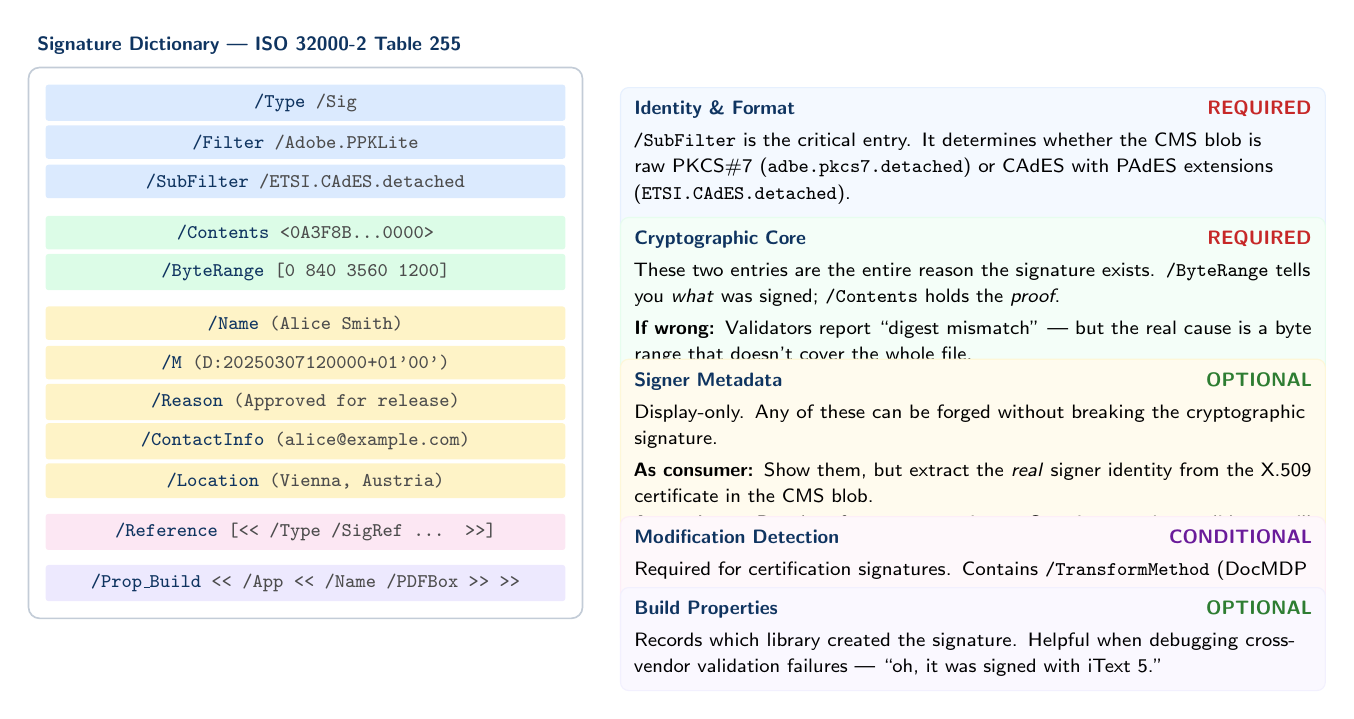
\begin{tikzpicture}[
    entry/.style={
        rectangle, rounded corners=1pt,
        font=\fontsize{7.5}{9}\selectfont\ttfamily,
        minimum width=6.6cm, minimum height=0.42cm,
        anchor=west, inner xsep=5pt,
    },
    panel/.style={
        rectangle, rounded corners=3pt,
        text width=8.6cm, font=\fontsize{7.5}{9.5}\selectfont\sffamily,
        inner sep=5pt, anchor=north west,
        line width=0.4pt,
    },
]

% ── Group A: Identity (blue) ───────────────────────────────────────────────
\node[entry, fill=groupA] (e1) at (0, 0)     {\textcolor{accent}{\textbf{/Type}}   \textcolor{black!70}{/Sig}};
\node[entry, fill=groupA] (e2) at (0,-0.50)  {\textcolor{accent}{\textbf{/Filter}} \textcolor{black!70}{/Adobe.PPKLite}};
\node[entry, fill=groupA] (e3) at (0,-1.00)  {\textcolor{accent}{\textbf{/SubFilter}} \textcolor{black!70}{/ETSI.CAdES.detached}};

% ── Group B: Crypto (green) ────────────────────────────────────────────────
\node[entry, fill=groupB] (e4) at (0,-1.65)  {\textcolor{accent}{\textbf{/Contents}} \textcolor{black!70}{<0A3F8B...0000>}};
\node[entry, fill=groupB] (e5) at (0,-2.15)  {\textcolor{accent}{\textbf{/ByteRange}} \textcolor{black!70}{[0 840 3560 1200]}};

% ── Group C: Metadata (amber) ─────────────────────────────────────────────
\node[entry, fill=groupC] (e6)  at (0,-2.80) {\textcolor{accent}{\textbf{/Name}}    \textcolor{black!70}{(Alice Smith)}};
\node[entry, fill=groupC] (e7)  at (0,-3.30) {\textcolor{accent}{\textbf{/M}}       \textcolor{black!70}{(D:20250307120000+01'00')}};
\node[entry, fill=groupC] (e8)  at (0,-3.80) {\textcolor{accent}{\textbf{/Reason}}  \textcolor{black!70}{(Approved for release)}};
\node[entry, fill=groupC] (e9)  at (0,-4.30) {\textcolor{accent}{\textbf{/ContactInfo}} \textcolor{black!70}{(alice@example.com)}};
\node[entry, fill=groupC] (e10) at (0,-4.80) {\textcolor{accent}{\textbf{/Location}} \textcolor{black!70}{(Vienna, Austria)}};

% ── Group D: Modification detection (pink) ─────────────────────────────────
\node[entry, fill=groupD] (e11) at (0,-5.45) {\textcolor{accent}{\textbf{/Reference}} \textcolor{black!70}{[<< /Type /SigRef ... >>]}};

% ── Group E: Build info (purple) ───────────────────────────────────────────
\node[entry, fill=groupE] (e12) at (0,-6.10) {\textcolor{accent}{\textbf{/Prop\_Build}} \textcolor{black!70}{<< /App << /Name /PDFBox >> >>}};

% ── Color-matched panels on the right ──────────────────────────────────────
\node[panel, fill=groupA!30, draw=groupA!70] (p1) at (7.3, 0.2) {
    \textbf{\textcolor{accent}{Identity \& Format}}
    \hfill\textcolor{reqcolor}{\scriptsize\textbf{REQUIRED}}\\[2pt]
    \texttt{/SubFilter} is the critical entry. It determines whether the CMS blob
    is raw PKCS\#7 (\texttt{adbe.pkcs7.detached}) or CAdES with PAdES extensions
    (\texttt{ETSI.CAdES.detached}).\\[2pt]
    \textbf{As producer:} Always use \texttt{ETSI.CAdES.detached} for new signatures.\\
    \textbf{As consumer:} Support all three SubFilters — legacy PDFs are everywhere.
};

\node[panel, fill=groupB!30, draw=groupB!70] (p2) at (7.3, -1.45) {
    \textbf{\textcolor{accent}{Cryptographic Core}}
    \hfill\textcolor{reqcolor}{\scriptsize\textbf{REQUIRED}}\\[2pt]
    These two entries are the entire reason the signature exists.
    \texttt{/ByteRange} tells you \emph{what} was signed;
    \texttt{/Contents} holds the \emph{proof}.\\[2pt]
    \textbf{If wrong:} Validators report ``digest mismatch'' — but the real cause is
    a byte range that doesn't cover the whole file.\\
    \textbf{Fix:} Verify \texttt{range1 + range2 + hex\_length == file\_size}.
};

\node[panel, fill=groupC!30, draw=groupC!70] (p3) at (7.3, -3.25) {
    \textbf{\textcolor{accent}{Signer Metadata}}
    \hfill\textcolor{optcolor}{\scriptsize\textbf{OPTIONAL}}\\[2pt]
    Display-only. Any of these can be forged without breaking the cryptographic
    signature.\\[2pt]
    \textbf{As consumer:} Show them, but extract the \emph{real} signer identity from
    the X.509 certificate in the CMS blob.\\
    \textbf{As producer:} Populate for user convenience. Security-conscious validators
    will ignore them anyway.
};

\node[panel, fill=groupD!30, draw=groupD!70] (p4) at (7.3, -5.25) {
    \textbf{\textcolor{accent}{Modification Detection}}
    \hfill\textcolor{condcolor}{\scriptsize\textbf{CONDITIONAL}}\\[2pt]
    Required for certification signatures. Contains \texttt{/TransformMethod}
    (DocMDP or FieldMDP) that constrains what changes are allowed after signing.
    Omit for plain approval signatures.
};

\node[panel, fill=groupE!30, draw=groupE!70] (p5) at (7.3, -6.15) {
    \textbf{\textcolor{accent}{Build Properties}}
    \hfill\textcolor{optcolor}{\scriptsize\textbf{OPTIONAL}}\\[2pt]
    Records which library created the signature. Helpful when debugging
    cross-vendor validation failures — ``oh, it was signed with iText 5.''
};

% ── Dict frame ──────────────────────────────────────────────────────────────
\begin{scope}[on background layer]
    \node[fit=(e1)(e12), inner sep=6pt, draw=accent!25,
          rounded corners=4pt, line width=0.6pt] (frame) {};
    \node[above=1pt of frame.north west, anchor=south west,
          font=\fontsize{7}{8}\selectfont\sffamily\bfseries\color{accent}]
          {Signature Dictionary — ISO 32000-2 Table 255};
\end{scope}

\end{tikzpicture}

\vfill
\clearpage

% ═══════════════════════════════════════════════════════════════════════════════
% VARIANT C: Dark Code Block with Numbered Callout Markers
% ═══════════════════════════════════════════════════════════════════════════════
\subsection*{\sffamily\color{accent} Variant C — Dark Code Block with Numbered Callouts}

{\small The dictionary is rendered as a dark code block with syntax highlighting.
Circled numbers in the margin mark points of interest, decoded in panels on the right.}

\vspace{0.6em}

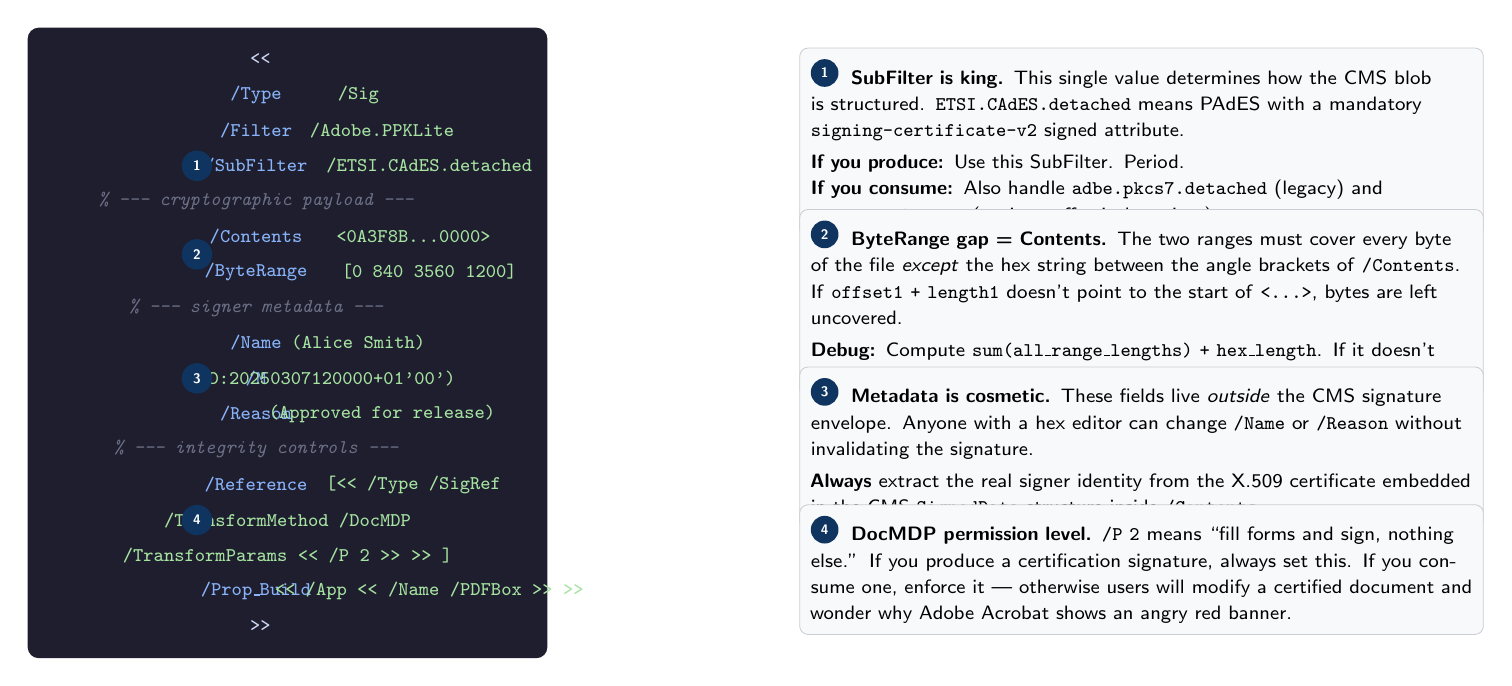
\begin{tikzpicture}[
    codeline/.style={
        anchor=west, font=\fontsize{7.5}{10}\selectfont\ttfamily, text=dicttext,
    },
    k/.style={text=keycolor, font=\fontsize{7.5}{10}\selectfont\ttfamily\bfseries},
    v/.style={text=valcolor, font=\fontsize{7.5}{10}\selectfont\ttfamily},
    c/.style={text=commentcolor, font=\fontsize{7.5}{10}\selectfont\ttfamily\itshape},
    callout/.style={
        circle, fill=accent, text=white,
        font=\fontsize{5.5}{6}\selectfont\bfseries\sffamily,
        minimum size=11pt, inner sep=0pt,
    },
    explain/.style={
        rectangle, rounded corners=3pt,
        fill=annobg, draw=annoframe, line width=0.3pt,
        text width=8.4cm, font=\fontsize{7.5}{9.5}\selectfont\sffamily,
        inner sep=4pt, anchor=north west,
    },
    enumcirc/.style={
        circle, fill=accent, text=white,
        font=\fontsize{5.5}{6}\selectfont\bfseries\sffamily,
        minimum size=10pt, inner sep=0pt,
    },
]

% ── Code block entries ──────────────────────────────────────────────────────
\def\codeX{0.4}
\def\lineH{0.45}

\node[codeline] (l0)  at (\codeX, 0)           {<<};

\node[k] at (\codeX+0.2, -1*\lineH)            {/Type};
\node[v] at (\codeX+1.5, -1*\lineH)            {/Sig};

\node[k] at (\codeX+0.2, -2*\lineH)            {/Filter};
\node[v] at (\codeX+1.8, -2*\lineH)            {/Adobe.PPKLite};

\node[k] (sf) at (\codeX+0.2, -3*\lineH)       {/SubFilter};
\node[v] at (\codeX+2.4, -3*\lineH)            {/ETSI.CAdES.detached};

\node[c] at (\codeX+0.2, -4*\lineH)            {\% --- cryptographic payload ---};

\node[k] at (\codeX+0.2, -5*\lineH)            {/Contents};
\node[v] at (\codeX+2.2, -5*\lineH)            {<0A3F8B...0000>};

\node[k] at (\codeX+0.2, -6*\lineH)            {/ByteRange};
\node[v] (br) at (\codeX+2.4, -6*\lineH)       {[0 840 3560 1200]};

\node[c] at (\codeX+0.2, -7*\lineH)            {\% --- signer metadata ---};

\node[k] at (\codeX+0.2, -8*\lineH)            {/Name};
\node[v] at (\codeX+1.5, -8*\lineH)            {(Alice Smith)};

\node[k] at (\codeX+0.2, -9*\lineH)            {/M};
\node[v] at (\codeX+1.1, -9*\lineH)            {(D:20250307120000+01'00')};

\node[k] at (\codeX+0.2, -10*\lineH)           {/Reason};
\node[v] (rs) at (\codeX+1.8, -10*\lineH)      {(Approved for release)};

\node[c] at (\codeX+0.2, -11*\lineH)           {\% --- integrity controls ---};

\node[k] at (\codeX+0.2, -12*\lineH)           {/Reference};
\node[v] at (\codeX+2.2, -12*\lineH)           {[<< /Type /SigRef};
\node[v] at (\codeX+0.6, -13*\lineH)           {/TransformMethod /DocMDP};
\node[v] (dm) at (\codeX+0.6, -14*\lineH)      {/TransformParams << /P 2 >> >> ]};

\node[k] at (\codeX+0.2, -15*\lineH)           {/Prop\_Build};
\node[v] at (\codeX+2.4, -15*\lineH)           {<< /App << /Name /PDFBox >> >>};

\node[codeline] (lend) at (\codeX, -16*\lineH) {>>};

% ── Dark background ────────────────────────────────────────────────────────
\begin{scope}[on background layer]
    \node[rectangle, rounded corners=4pt, fill=dictbg,
          fit=(l0)(lend)(dm), inner xsep=8pt, inner ysep=6pt,
          minimum width=6.6cm] (bg) {};
\end{scope}

% ── Callout markers (in left margin of code block) ─────────────────────────
\node[callout] (c1) at (-0.15, -3*\lineH)   {1};
\node[callout] (c2) at (-0.15, -5.5*\lineH) {2};
\node[callout] (c3) at (-0.15, -9*\lineH)   {3};
\node[callout] (c4) at (-0.15, -13*\lineH)  {4};

% ── Explanation panels on the right ─────────────────────────────────────────
\node[explain] (e1) at (7.5, 0.15) {
    \raisebox{-1pt}{\tikz\node[enumcirc]{1};}\;
    \textbf{SubFilter is king.} This single value determines how the CMS blob
    is structured. \texttt{ETSI.CAdES.detached} means PAdES with a mandatory
    \texttt{signing-certificate-v2} signed attribute.\\[2pt]
    \textbf{If you produce:} Use this SubFilter. Period.\\
    \textbf{If you consume:} Also handle \texttt{adbe.pkcs7.detached}
    (legacy) and \texttt{adbe.pkcs7.sha1} (ancient, effectively extinct).
};

\node[explain] (e2) at (7.5, -1.9) {
    \raisebox{-1pt}{\tikz\node[enumcirc]{2};}\;
    \textbf{ByteRange gap = Contents.} The two ranges must cover every byte
    of the file \emph{except} the hex string between the angle brackets of
    \texttt{/Contents}. If \texttt{offset1 + length1} doesn't point to
    the start of \texttt{<...>}, bytes are left uncovered.\\[2pt]
    \textbf{Debug:} Compute \texttt{sum(all\_range\_lengths) + hex\_length}.
    If it doesn't equal the file size, the signature is incomplete.
};

\node[explain] (e3) at (7.5, -3.9) {
    \raisebox{-1pt}{\tikz\node[enumcirc]{3};}\;
    \textbf{Metadata is cosmetic.} These fields live \emph{outside} the CMS
    signature envelope. Anyone with a hex editor can change \texttt{/Name}
    or \texttt{/Reason} without invalidating the signature.\\[2pt]
    \textbf{Always} extract the real signer identity from the X.509 certificate
    embedded in the CMS \texttt{SignedData} structure inside \texttt{/Contents}.
};

\node[explain] (e4) at (7.5, -5.65) {
    \raisebox{-1pt}{\tikz\node[enumcirc]{4};}\;
    \textbf{DocMDP permission level.} \texttt{/P 2} means ``fill forms and sign,
    nothing else.'' If you produce a certification signature, always set this.
    If you consume one, enforce it — otherwise users will modify a certified
    document and wonder why Adobe Acrobat shows an angry red banner.
};

\end{tikzpicture}

\vfill

\begin{center}
\small\sffamily\color{commentcolor}
\textit{End of test variants — choose one (or combine elements) for the book style.}
\end{center}

\end{document}
